\documentclass[11pt]{article}

\usepackage[a4paper,margin=2.4cm]{geometry}
\usepackage{amsmath}
\usepackage{amssymb}
\usepackage{graphicx}
\usepackage{booktabs}
\usepackage{caption}
\usepackage[hidelinks]{hyperref}
\usepackage{microtype}

\captionsetup{font=small,labelfont=bf}
\setlength{\parskip}{0.4em}

\title{\vspace{-1.5cm}\textbf{Reducing CO$_2$ Levels Using Genetic Algorithms:\\A Re-evaluation}}
\author{Cristian Lincu}
\date{}

\begin{document}
\maketitle
\vspace{-1cm}

\begin{abstract}
\noindent
This project provides a solution framework for minimizing CO$_2$ emission
levels in a national power grid through machine learning methods. The data is
collected via Energinet's public API, which provides real-time data about
Denmark's power system. The framework retains the structure of the original
formulation --- a regression model inferring CO$_2$ levels, gradient-boosted
regressors forecasting demand and renewable production, and a genetic
ensemble searching for the emission-minimizing distribution --- while
correcting a set of modelling errors that made the original results
unreliable. The central correction is that the optimizer was previously able
to exploit its own surrogate: an unconstrained regression tree, fitted to
confounded data, reported that emissions \emph{fall} when thermal generation
rises, and the genetic heuristic duly proposed ramping thermal plants. This
work constrains the emissions model to be physically monotone, evaluates every
component chronologically rather than on shuffled splits, replaces
scale-invariant coherence with explicit ramp limits, and measures the
optimizer against the counterfactual in which dispatch is held fixed. The
resulting system proposes feasible four-hour dispatch trajectories that reduce
CO$_2$ intensity by approximately 55\% relative to that counterfactual.
\end{abstract}

\section{Introduction}

The data is collected via Energinet's public
API\footnote{\url{https://www.energidataservice.dk/tso-electricity/PowerSystemRightNow}}
which provides real-time data about Denmark's power system. The dataset
prepared for this research consists of one year of records aggregated onto the
15-minute grid used for imbalance settlement in Denmark, giving 34{,}600
observations between September 2025 and September 2026.

The main elements of this project are: a regression model for inferring
CO$_2$ levels, XGBoost regressors for predicting demand and renewable energy
production, and genetic algorithms for finding the optimal energy distribution
with respect to CO$_2$ emission minimization. The goal is to infer the optimal
resource combinations that minimize CO$_2$ emissions, depending on future
demand and renewables production.

This paper is a re-evaluation of an earlier version of the same framework.
The earlier version reported potential emission reductions of 50--75\%. Those
figures did not survive scrutiny, for reasons set out in
Section~\ref{sec:corrections}. The methodology below preserves as much of the
original design as the physics allows, and states plainly where it does not.

\section{Data and the energy balance}
\label{sec:data}

The national energy balance is the identity
\begin{equation}
D = \underbrace{P_{\ge 100} + P_{< 100} + R}_{\text{generation}} + \sum_{i \in \mathcal{B}} x_i ,
\label{eq:balance}
\end{equation}
where $R$ denotes renewable production (solar and wind), $P_{\ge 100}$ and
$P_{< 100}$ denote energy produced by power plants with installed capacity
greater or equal to 100~MW and less than 100~MW respectively, and
$\mathcal{B}$ is the set of \emph{cross-border} interconnectors: DK1-DE,
DK1-NL, DK1-GB, DK1-NO, DK1-SE, DK2-DE, DK2-SE and Bornholm-SE. Positive
exchange values are imports, negative ones are exports.

The DK1-DK2 link is deliberately absent from $\mathcal{B}$. It is the Great
Belt Power Link, which joins the two Danish bidding zones; power flowing
across it is internal and cannot change national supply. Energinet excludes it
from its own \texttt{Exchange\_Sum} field for precisely this reason, which is
verifiable directly from the API: on an arbitrary record the eight
cross-border flows sum to 3481.49~MW and \texttt{Exchange\_Sum} reports
3481.49~MW, with the DK1-DK2 value of $-371.57$~MW sitting outside the total.
The original formulation included DK1-DK2 in the balance, displacing demand by
up to 600~MW against a tolerance of 1\% of demand. It remains a decision
variable, because it carries zonal information the emissions model uses, but
it no longer contributes to Equation~\eqref{eq:balance}.

\section{Methodology}

\subsection{I. Inferring CO\texorpdfstring{$_2$}{2} levels}
\label{sec:co2}

A regression model infers CO$_2$ levels taking into account 12 features:
renewable energy production (solar and wind), energy produced by power plants
with installed capacity greater or equal to 100~MW, energy produced by power
plants with installed capacity less than 100~MW, and the nine energy exchanges
between Denmark and other countries or areas. The hyperparameters are tuned
using randomized search, and the model is evaluated through time-series
cross-validation.

Two changes to this component are essential rather than cosmetic.

\paragraph{The target is total emissions, not intensity.}
Energinet publishes CO$_2$ as an intensity in g/kWh. Modelling intensity
directly is what allowed the original surrogate to be exploited, because
intensity is confounded: in Denmark, hours with high output from large thermal
plants are also hours with high wind, so an unconstrained model learns that
thermal generation predicts \emph{low} emissions. The model here predicts the
total emission rate
\begin{equation}
\Theta = \frac{\text{CO}_2\text{ intensity} \times D}{1000} \quad [\mathrm{t/h}],
\end{equation}
from which intensity is recovered as $1000\,\Theta / D$. Under
consumption-based accounting every supply source carries a non-negative
emission factor, so total emissions are monotonically non-decreasing in every
source. That is imposed as a hard constraint on all eleven controllable
features. Renewables are left unconstrained, since they are not a decision
variable.

\paragraph{The estimator is an ensemble, and it reports its own reliability.}
A single constrained regression tree lacks the capacity to fit the data
without leaning on the confound, so the deployed estimator is a
gradient-boosted ensemble of regression trees carrying the same monotonicity.
A companion depth-capped tree partitions the feature space and supplies, for
any candidate, the number of training observations $n(\mathbf{x})$ behind its
leaf and the dispersion $\sigma(\mathbf{x})$ of the target within it. A
Mahalanobis distance $d^2(\mathbf{x})$ to the training distribution measures
how far a candidate sits from anything ever observed. Both quantities enter
the fitness function, so the optimizer is penalized for leaving the region
where the model has evidence.

\subsection{II. Forecasting demand and renewable production}

The XGBoost regressors provide multi-step forecasting for energy demand and
renewable production over the next 16 time points, that is four hours ahead at
15-minute resolution. These forecasts are important because the optimal power
distribution has to match demand continuously; a persistent mismatch between
supply and demand is what a system operator resolves through reserves, and the
schedule the optimizer proposes must not create one. The distributable energy
whose allocation is optimized is the difference between forecasted demand and
forecasted renewable energy, $D_{XG} - R_{XG}$.

Renewable production is no longer extrapolated from its own recent output.
Wind four hours ahead is not recoverable from the last few observations, and
attempting it was the weakest part of the original system. Instead the model
consumes Energinet's own physical forecast and learns a correction on top of
it. The \texttt{Forecast5Hour} vintage is issued approximately five hours
before its target and is therefore genuinely available at decision time across
the whole horizon, which keeps the evaluation free of look-ahead.

Every model is trained on a chronological split and reported against a
persistence baseline, and the renewables model additionally against the raw
Energinet forecast it post-processes.

\subsection{III. Genetic optimization of a dispatch trajectory}

For the forecasted horizon, the optimal combination of sources is inferred
using genetic algorithms. In order to escape eventual local optima and
increase the method's success, this is done by employing a genetic ensemble
with 16 optimizers. Populations of solutions are initialized stochastically
and transformed by evolutionary processes to arrive at the ``fittest''
distribution. The restrictions are the ranges of power plant production and
the interconnector limits for exchanges, inferred from the past year's data
and capped by technical transfer capacity. Ramp limits are taken from the
99th percentile of realised 15-minute changes over the same year, which
describes what the fleet can actually do better than any fixed assumption.
At 1~MW resolution a single time step admits approximately $8 \times 10^{34}$
combinations.

\paragraph{A chromosome is a trajectory.}
In the original formulation each forecasted time point was optimized
independently, and coherence between consecutive solutions was encouraged by a
cosine-similarity term. Cosine similarity is scale invariant --- two
distributions differing by a factor of ten have similarity 1 --- so it could
not constrain magnitudes, and in the deployed system it did not: consecutive
five-minute solutions differed by more than 1{,}100~MW on a single
interconnector. Here a chromosome is the whole trajectory. Writing $d = 11$
for the number of genes per time step and $T = 16$ for the horizon, each
individual is a matrix $X^{(j)} \in \mathbb{R}^{T \times d}$ whose rows
$x^{(j)}_t$ are the distributions at each step, and the first generation is
\begin{equation}
G =
\begin{bmatrix}
- & \operatorname{vec}(X^{(1)}) & - \\
- & \operatorname{vec}(X^{(2)}) & - \\
  & \vdots &   \\
- & \operatorname{vec}(X^{(m)}) & -
\end{bmatrix} \in \mathbb{R}^{m \times Td},
\end{equation}
where $m$ is the size of the population. Coherence is then imposed directly,
as a ramp constraint between consecutive rows, rather than hoped for through a
similarity term.

\paragraph{The fitness function.}
Each chromosome is evaluated using the regression ensemble to infer the
CO$_2$ emission level implied by the solution it represents, while solutions
that do not balance the power grid are penalized by an augmentation that
significantly reduces their coupling chances. Each optimal trajectory
minimizes
\begin{equation}
X^{*} = \underset{X^{(j)}}{\operatorname{argmin}} \;
\frac{1}{T}\sum_{t=1}^{T}
\Big[\,
\xi_b\, \mathcal{P}_b(x_t) \;+\;
\xi_r\, \mathcal{P}_r(x_t, x_{t-1}) \;+\;
\xi_s\, \mathcal{P}_s(x_t) \;+\;
\zeta\, \Theta(x_t) \;+\;
\gamma\, \sigma(x_t)
\,\Big],
\label{eq:fitness}
\end{equation}
whose terms are, in order,

\begin{itemize}
\itemsep0.15em
\item the \textbf{grid imbalance penalty}
\begin{equation}
\mathcal{P}_b(x_t) = \mathbf{I}\!\left(\left|D_{XG,t} - R_{XG,t} - \sum_{i \in \mathcal{B}} x_{t,i}\right| > \tau D_{XG,t}\right)
\left(1 + \frac{\left|D_{XG,t} - R_{XG,t} - \sum_{i \in \mathcal{B}} x_{t,i}\right|}{\tau D_{XG,t}}\right),
\end{equation}
where $\mathbf{I}$ is the indicator function, $D_{XG}$ is the demand forecast
and $R_{XG}$ the renewable forecast provided by the XGBoost regressors, and
$\tau = 0.01$. The indicator alone, as used originally, produces a flat
plateau that a heuristic cannot descend; scaling it by the relative size of
the violation gives the search a gradient towards feasibility while preserving
the hard threshold;

\item the \textbf{ramp penalty}
$\mathcal{P}_r(x_t, x_{t-1}) = \sum_{i} \max\!\left(0, |x_{t,i} - x_{t-1,i}| - \rho_i\right)/\rho_i$,
with $\rho_i$ the per-resource ramp limit and $x_0$ the latest observed
distribution. This term replaces the cosine similarity of the original
formulation and performs the role that term was intended to perform;

\item the \textbf{support penalty}
$\mathcal{P}_s(x_t) = \mathbf{I}\!\left(n(x_t) < n_{\min}\right) + \max\!\left(0, d^2(x_t)/d^2_{q} - 1\right)$,
which confines the search to the region where the emissions model has
evidence, with $n_{\min} = 20$ and $d^2_q$ the 99th percentile of the training
Mahalanobis distances;

\item the \textbf{emissions level} $\Theta$ inferred by the regression
ensemble, augmented by $\zeta$; and

\item the \textbf{model dispersion} $\sigma$, augmented by $\gamma$, which
makes the optimizer prefer solutions the model is confident about.
\end{itemize}

\paragraph{Feasibility by construction.}
Every candidate is passed through a repair operator before evaluation. Walking
the horizon forward, the admissible box at each step is the intersection of
the technical limits with the ramp window around the previous step; the
residual energy imbalance is then distributed across the balance-carrying
resources in proportion to their remaining headroom. This turns feasibility
from something the search must rediscover into a property of the
representation, so the evolutionary effort is spent on emissions instead.

\paragraph{Implementation.}
The ensemble of independent optimizers is evaluated as a single batched array,
an island model with periodic migration of the best individual between
islands. Emissions, dispersion, leaf support and novelty all come out of one
traversal per generation. With 16 islands, populations of 150 and 200
generations --- $4.8\times10^{5}$ evaluations --- a full solve takes
approximately 57 seconds, which fits comfortably inside a scheduled job
refreshing every 30 minutes.

\section{Results}

\subsection{The emissions model}

Table~\ref{tab:co2} reports the emissions model against the original
formulation on identical data. Two comparisons matter. The original tree
evaluated with a shuffled split achieves 5.77~g/kWh, but a shuffled split on a
15-minute series places near-duplicate neighbours on both sides of the
partition; evaluated chronologically, the same model achieves 13.01~g/kWh. The
constrained ensemble achieves 11.05~g/kWh --- better than the original
managed under honest evaluation, while additionally being physically valid.

\begin{table}[h]
\centering
\small
\begin{tabular}{lccc}
\toprule
Model & Evaluation & Intensity MAE (g/kWh) & Monotone \\
\midrule
Fully grown tree, intensity & shuffled split & 5.77 & no \\
Fully grown tree, intensity & chronological & 13.01 & no \\
Monotone ensemble, total emissions & chronological & \textbf{11.05} & yes \\
\bottomrule
\end{tabular}
\caption{CO$_2$ model accuracy. The shuffled-split figure is reported because
it is what the original framework published; it is inflated by leakage between
adjacent observations.}
\label{tab:co2}
\end{table}

Figure~\ref{fig:probe} shows why the constraint matters more than the accuracy.
Holding every other resource fixed and sweeping large-plant output from 0 to
1500~MW, the original model reports total emissions falling to a minimum at
300~MW before rising. A genetic algorithm minimizing that surface will ramp
thermal generation, which is exactly what the deployed system did. The
constrained model is monotone by construction and its minimum is at zero.

\begin{figure}[h]
\centering
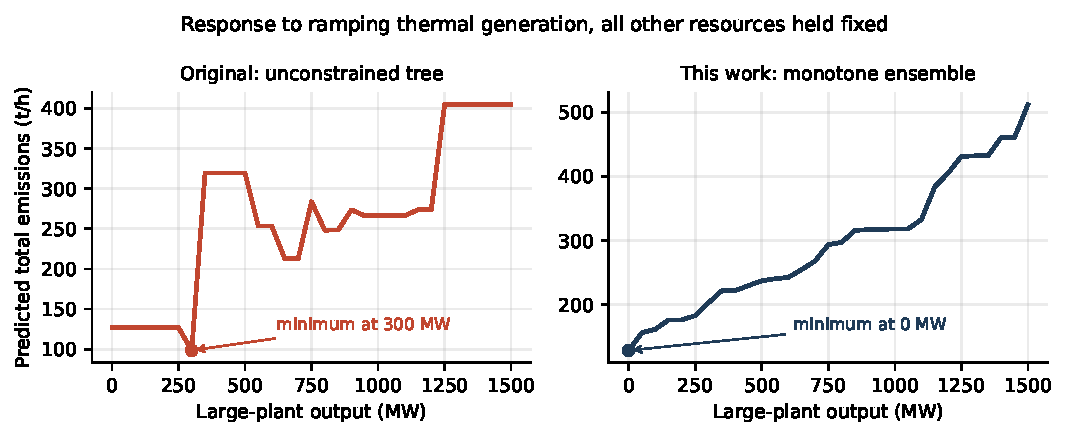
\includegraphics[width=\textwidth]{figures/probe.pdf}
\caption{Response of each emissions model to ramping thermal generation with
all other resources held fixed. The original model rewards the optimizer for
starting thermal plants.}
\label{fig:probe}
\end{figure}

\subsection{The forecasts}

Figure~\ref{fig:forecast} reports forecast error against horizon on a
chronological hold-out. Demand RMSE grows from 88.9~MW at 15 minutes to
374.5~MW at four hours, against a persistence baseline of 98.3~MW and
815.8~MW. Renewables RMSE grows from 135.9~MW to 468.6~MW, against 151.7~MW
and 1394.0~MW for persistence and a flat 699.5~MW for the raw Energinet
forecast; post-processing that forecast with recent observations improves on
it at every horizon.

\begin{figure}[h]
\centering
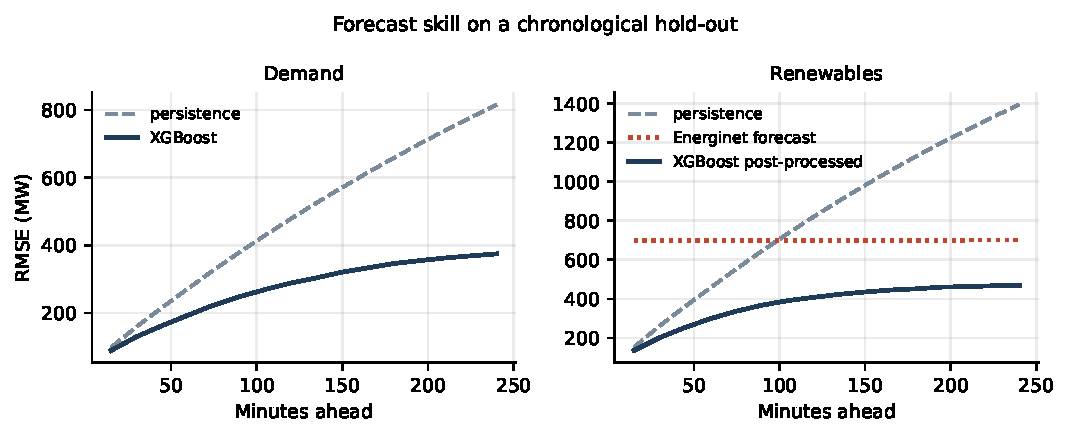
\includegraphics[width=\textwidth]{figures/forecast_skill.pdf}
\caption{Forecast skill against horizon, with baselines.}
\label{fig:forecast}
\end{figure}

\subsection{The optimizer}

An evolutionary heuristic is only worth its cost if it beats random search
under the same evaluation budget. Figure~\ref{fig:convergence} shows that it
does: at $4.8\times10^{5}$ evaluations and matched wall-clock time, the
genetic ensemble reaches a mean intensity of 60.8~g/kWh against 87.7~g/kWh for
random search, and does so while keeping every step inside the region where
the emissions model has support, which random search does not.

\begin{figure}[h]
\centering
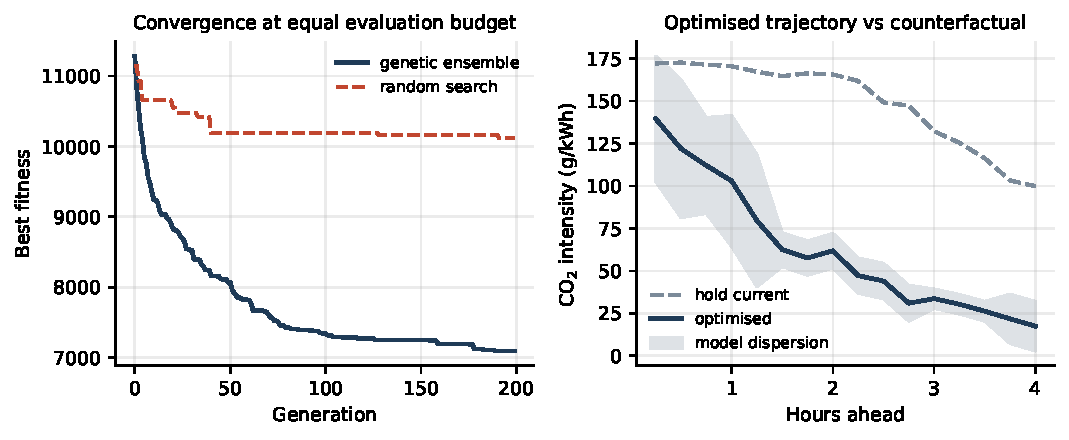
\includegraphics[width=\textwidth]{figures/convergence.pdf}
\caption{Left: convergence against random search at equal evaluation budget.
Right: the optimized intensity trajectory against the hold-current
counterfactual, with the emissions model's own dispersion shaded.}
\label{fig:convergence}
\end{figure}

\subsection{How the reduction is measured}
\label{sec:attribution}

The original framework compared optimized future emissions against the
\emph{present} measured value. That comparison credits the optimizer with
whatever the weather was going to do anyway: if wind is rising over the
horizon, intensity falls without any intervention at all.

The reduction reported here is measured against a hold-current counterfactual,
in which demand and renewables follow their forecasts but the controllable
resources stay where they are. On the representative solve shown in
Figure~\ref{fig:dispatch}, the present measured intensity was 204.1~g/kWh, the
counterfactual averaged 140.0~g/kWh over the horizon, and the optimized
trajectory averaged 63.8~g/kWh. The honest reduction attributable to
re-dispatch is therefore 54.4\%, not the 68.7\% that comparison against the
present value would have produced.

\begin{figure}[h]
\centering
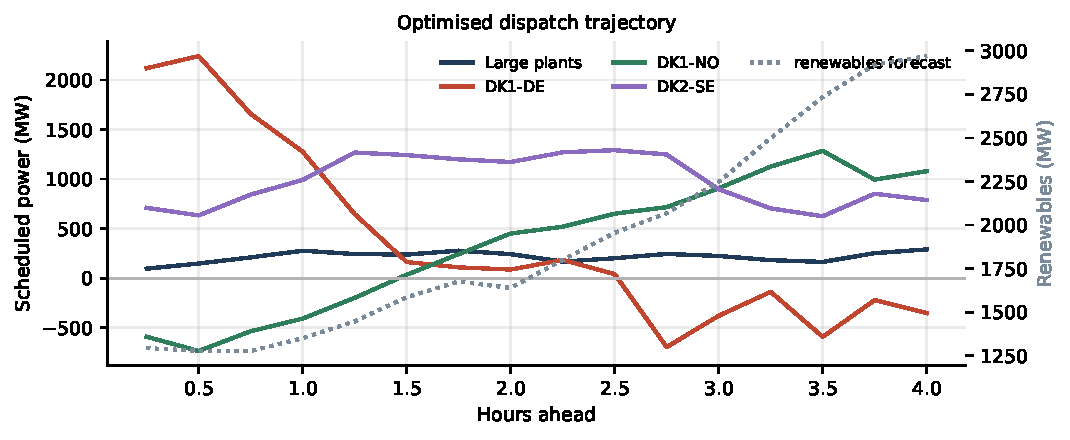
\includegraphics[width=\textwidth]{figures/dispatch.pdf}
\caption{An optimized dispatch trajectory. As forecast wind rises through the
afternoon the schedule withdraws from German imports, crossing into export,
and shifts towards Norwegian hydro, while thermal output stays low. Every
change respects its ramp limit.}
\label{fig:dispatch}
\end{figure}

The trajectory itself is physically legible, which the original solutions were
not. Every step satisfies the energy balance to within a fraction of a
megawatt and every change respects its ramp limit; the maximum balance error
over the horizon is $2.4\times10^{-4}$~MW.

\section{What changed relative to the original formulation}
\label{sec:corrections}

\begin{table}[h]
\centering
\small
\begin{tabular}{p{5.4cm}p{9.4cm}}
\toprule
Issue & Correction \\
\midrule
Optimizer exploited its own surrogate & Emissions model constrained monotone in every supply source; target changed from intensity to total emissions \\
Fully grown tree acted as a lookup table & Depth- and leaf-capped boosted ensemble; 25{,}863 leaves reduced to a bounded ensemble \\
No guard against unseen combinations & Leaf support and Mahalanobis novelty penalties in the fitness function \\
Shuffled splits on a time series & Chronological splits and time-series cross-validation throughout, with persistence baselines \\
Cosine similarity used for coherence & Explicit per-resource ramp limits derived from observed 15-minute changes \\
DK1-DK2 counted in the national balance & Restricted to the eight cross-border links, matching Energinet's own convention \\
Results clamped so they could not look worse than the status quo & Removed; the counterfactual is published alongside the optimized result \\
Reduction measured against present emissions & Measured against the hold-current counterfactual over the same horizon \\
Independent per-step optimization & Trajectory chromosome with coupled ramp constraints \\
Search bounds fixed and stale & Bounds and ramp limits re-derived from the training year, capped by technical capacity \\
\bottomrule
\end{tabular}
\caption{Corrections applied to the original framework.}
\end{table}

Two further errors are worth recording because they were silent. The
\texttt{PowerSystemRightNow} schema changed after the original models were
trained: the \texttt{ImbalanceDK1}, \texttt{ImbalanceDK2} and
\texttt{mFRRActivated} fields no longer exist. The original notebooks selected
features by position, so the same code now silently selects different columns.
All feature selection here is by name. Separately, the deployed pipeline used
a selection-pressure parameter of 150 where the notebook that validated the
method used 8, which collapses the population to near-clones of a single
individual within a few generations.

\section{Limitations}

The framework does not model unit commitment. Large-plant output is treated as
a single aggregate quantity, where in reality it is dozens of units with
individual minimum stable loads and start-up times.

Interconnector limits are fixed over the horizon. Real transfer capacities are
published per market time unit and are frequently derated; a production system
would consume them rather than assume them.

The model takes no account of exchange contract terms or energy prices, so a
proposed schedule may be physically feasible and economically impossible.

Most importantly, Energinet's CO$_2$ figure is a \emph{consumption-based}
intensity for Denmark: it assigns emission factors to imports. A schedule can
therefore lower the Danish number by importing more low-carbon power from
Norway or Sweden without lowering emissions anywhere. Nordic hydro export
capacity is finite, so power drawn to Denmark is power not delivered
elsewhere, and the displaced consumer may burn gas instead. The reductions
reported here are reductions in Denmark's attributed intensity. Establishing
how much of that is genuine abatement requires marginal emissions data for the
surrounding system, which is outside the scope of this work. This caveat
applies equally to the original framework, where it was not stated.

\section{Future work}

Future work for customizing this model to any power grid might take into
consideration other important aspects, like in-depth details about exchange
contract terms, to the extent of their availability, and energy prices, and
include them in the evaluation of solutions, extending the realism initiated
by the ramp constraints.

Three directions follow from the limitations above. Replacing average with
marginal emission factors would let the objective express abatement rather
than attribution. Introducing semi-continuous constraints for minimum stable
load would turn the problem into a genuine mixed-integer program, where the
choice of an evolutionary heuristic could be benchmarked against an exact
solver. And a systematic backtest, replaying historical periods and scoring
proposed dispatch against realised outcomes, would convert the results
reported here from a demonstration into evidence.

\vspace{0.6em}
\noindent\rule{\textwidth}{0.4pt}

\noindent\small
Visit the web app, which includes a dynamic comparison between recent
emissions in Denmark's power system, the hold-current counterfactual, and the
minimized CO$_2$ levels over the next four hours, as well as the optimal
energy resource distributions leading to these emission levels.

\end{document}
